\subsection{Nguồn 2: }
\subsubsection{Giới thiệu Dataset:}
Bộ dữ liệu này ghi lại xu hướng nghe nhạc trực tuyến toàn cầu trên Spotify trong năm 2024 được mô phỏng để phản ánh các xu hướng thực tế. Nguồn tham khảo bao gồm Spotify Wrapped 2023, IFPI Global Music Report, và Chartmetric. Nó mang đến những thông tin giá trị về sở thích của người dùng tại nhiều quốc gia, các nghệ sĩ và album nổi bật, tổng số giờ nghe nhạc, cũng như hành vi của người nghe. Được xây dựng nhằm phục vụ cho các mục đích như phân tích dữ liệu chuyên sâu, phát triển mô hình học máy, và xây dựng hệ thống báo cáo – bảng điều khiển thông minh trong lĩnh vực âm nhạc và truyền thông.\newline
Bộ dữ liệu $‘Spotify\_2024\_Global\_Streaming\_Data.csv‘$ gồm 500 dòng và 12 cột. Bao gồm các features sau:

\begin{table}[h!]
\centering
\renewcommand{\arraystretch}{1.2} % giãn dòng cho đẹp
\begin{tabularx}{\textwidth}{|>{\raggedright\arraybackslash}X|c|>{\raggedright\arraybackslash}X|}
\hline
\textbf{Column} & \textbf{Data type} & \textbf{Meaning} \\
\hline
Country & object  & Quốc gia ghi nhận dữ liệu nghe nhạc \\
\hline
Artist & object  & Tên nghệ sĩ hoặc ban nhạc \\
\hline
Album & object  & Tên album do nghệ sĩ phát hành \\
\hline
Genre & object  & Thể loại âm nhạc (ví dụ: Pop, Hip-hop, R\&B, Classical, ...) \\
\hline
Release Year & int64  & Năm album được phát hành chính thức \\
\hline
Monthly Listeners (Million) & float64 & Số lượng người nghe hàng tháng trung bình của nghệ sĩ (tính theo triệu) \\
\hline
Total Streams (Millions) & float64 & Tổng số lượt phát (lượt nghe) toàn cầu của album (tính theo triệu) \\
\hline
Total Hours Streamed (Millions) & float64 & Tổng thời gian người dùng đã nghe album \\
\hline
Avg Stream Duration (Min) & float64 & Thời lượng trung bình của 1 lượt nghe album \\
\hline
Platform Type & object & Loại tài khoản người dùng: Free hay Premium \\
\hline
Streams Last 30 Days & float64 & Tổng lượt nghe 30 ngày gần nhất của bài hát \\
\hline
Skip Rate (\%) & float64 & Tỉ lệ bỏ qua bài hát khi chưa nghe hết bài hát \\
\hline
\end{tabularx}
\caption{Thông tin features dữ liệu nghe nhạc}
\end{table}
\subsubsection{Data enrichment:}
Gọi Spotify Search API với album name + artist để lấy đúng album\_id. Với album\_id lấy được gọi Recobeats API để lấy thêm các features sau đây:
\begin{table}[h!]
\centering
\renewcommand{\arraystretch}{1.2} % giãn dòng
\begin{tabularx}{\textwidth}{|>{\raggedright\arraybackslash}X|c|>{\raggedright\arraybackslash}X|}
\hline
\textbf{Feature} & \textbf{Type} & \textbf{Meaning} \\
\hline
id & string & Reccobeats’ id, id duy nhất cho mỗi album \\
\hline
albumType & string & Kiểu album (album, single, compilation) \\
\hline
artist & object & Danh sách các nghệ sĩ tham gia album, id artist, href Spotify artist \\
\hline
totalTracks & integer & Tổng số track trong album \\
\hline
href & string & Spotify URL của album \\
\hline
name & string & Tên của album \\
\hline
availableCountries & string & Danh sách các quốc gia có sẵn cho album này, định danh bằng ISO 3166 alpha-2 code, phân biệt bởi dấu phẩy \\
\hline
releaseDate & string & Ngày phát hành đầu tiên \\
\hline
releaseDateFormat & string & Định dạng của ngày phát hành (day, month, year) \\
\hline
isrc & string & {\color[HTML]{1C1E21}International Standard Recording Code (Optional)} \\
\hline
ean & string & {\color[HTML]{1C1E21}European Article Number (Optional)} \\
\hline
upc & string & {\color[HTML]{1C1E21}Universal Product Code (Optional)} \\
\hline
label & string & Nhãn gắn với album (hashtag) \\
\hline
poppularity & integer & Độ nổi tiếng của album. Giá trị chạy từ 0–100, với 100 là giá trị nổi tiếng nhất \\
\hline
\end{tabularx}
\caption{Thông tin các trường dữ liệu album từ Reccobeats/Spotify}
\end{table}

\subsubsection{Data cleaning and preprocessing: }
Kiểm tra các dữ liệu bị thiếu, xác minh các kiểu dữ liệu:

\begin{figure}[H]
    \centering
    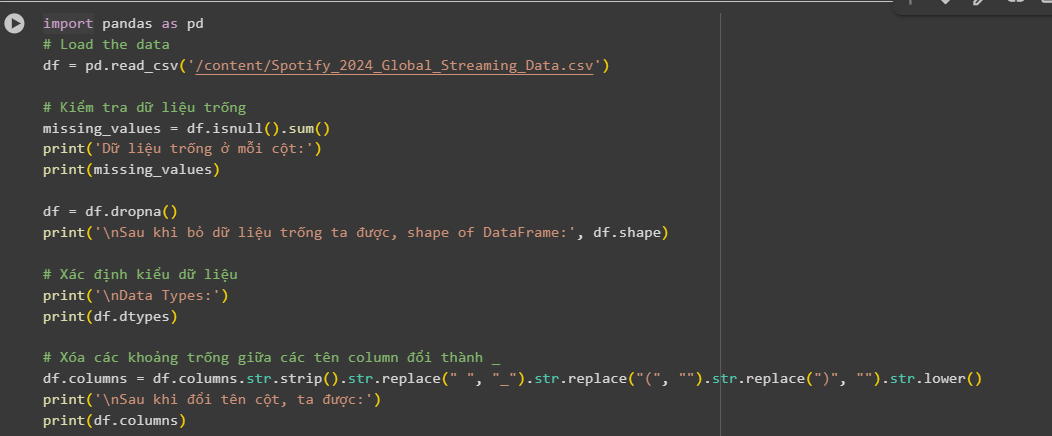
\includegraphics[width=1\linewidth]{../graphics/data2/1.png}
    \caption{Kiểm tra null, xác định kiểu dữ liệu và đổi các khoảng trống giữa các features}
    \label{fig:placeholder}
\end{figure}
\begin{figure}[H]
    \centering
    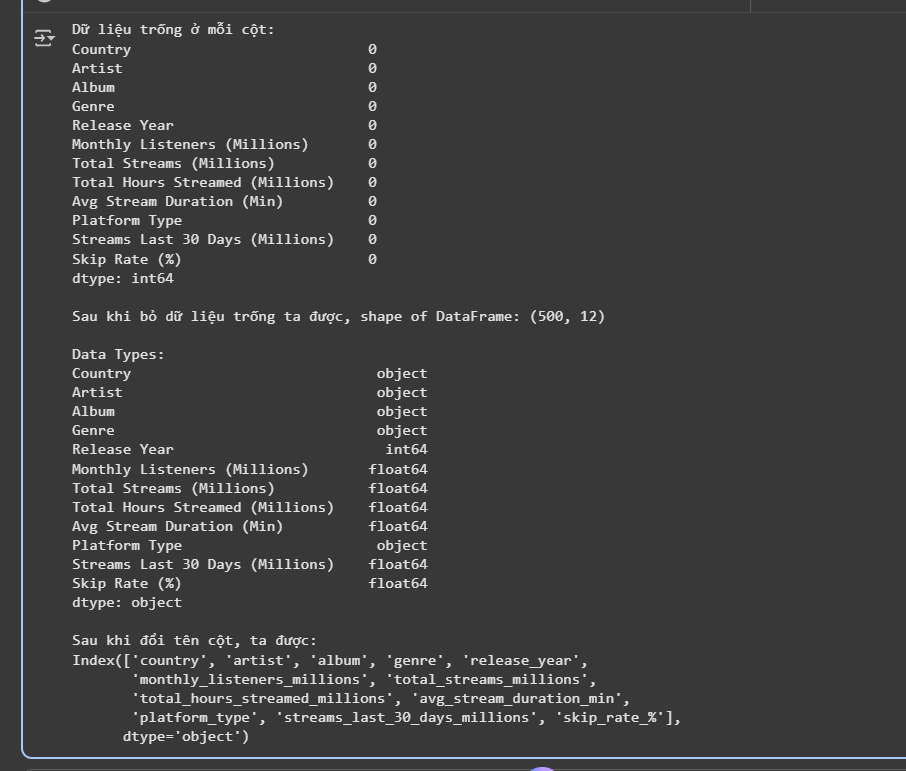
\includegraphics[width=0.8\linewidth]{../graphics/data2/2.png}
    \caption{KẾt quả từ hình 1}
    \label{fig:placeholder}
\end{figure}
Từ file dataset ban đầu ta gọi spotify api để lấy spotify\_id cho mỗi album được file ‘Albums\_Info\_Clean.csv’, từ đó gọi reccobeats api để lấy thêm các features, tạo thành 1 file mới là:

\begin{figure}[H]
    \centering
    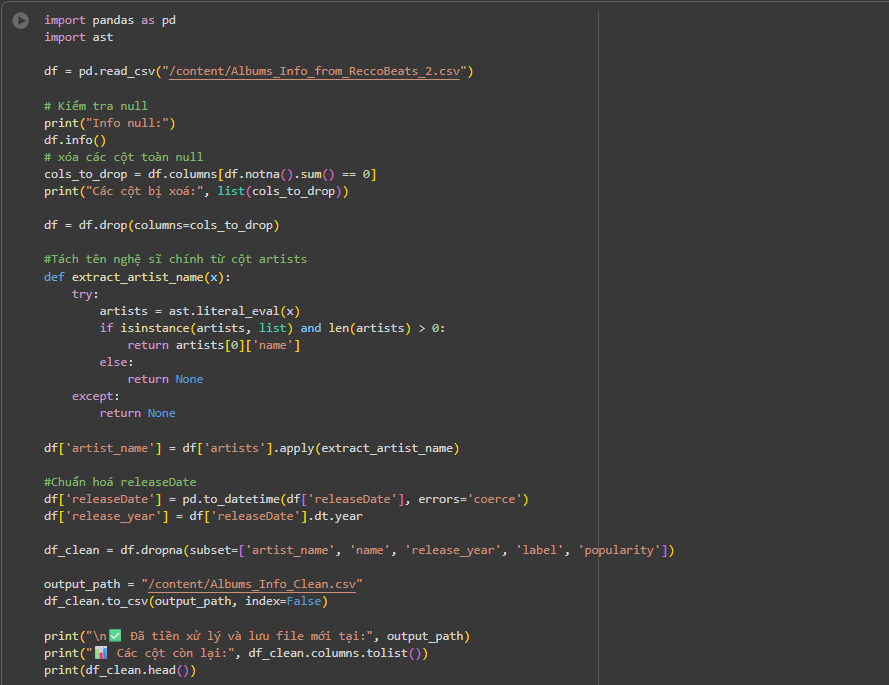
\includegraphics[width=0.9\linewidth]{../graphics/data2/4.png}
    \caption{Kiểm tra, xóa các cột null, tách tên nghệ sĩ và chuẩn hóa releaseDate}
    \label{fig:placeholder}
\end{figure}

\begin{figure}[H]
    \centering
    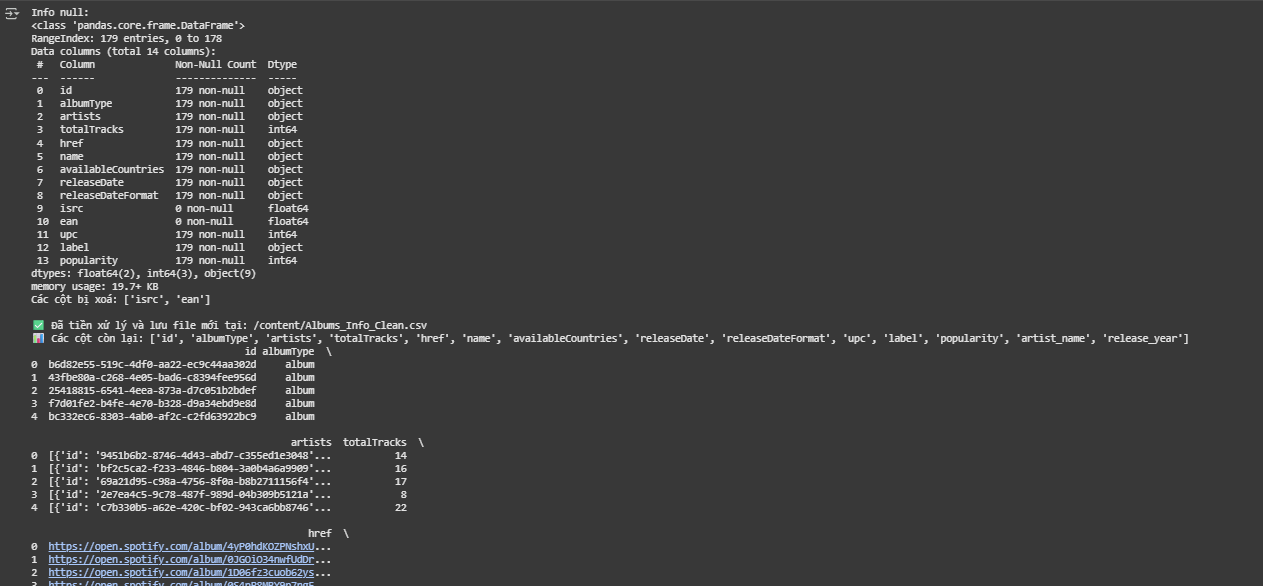
\includegraphics[width=0.9\linewidth]{../graphics/data2/5.png}
    \caption{Kết quả từ hình 3}
    \label{fig:placeholder}
\end{figure}


\subsubsection{Overview and Analysis}
\textbf{Dataset ban đầu Spotify\_2024\_Global\_Streaming\_Data.csv:}
\begin{figure}[H]
    \centering
    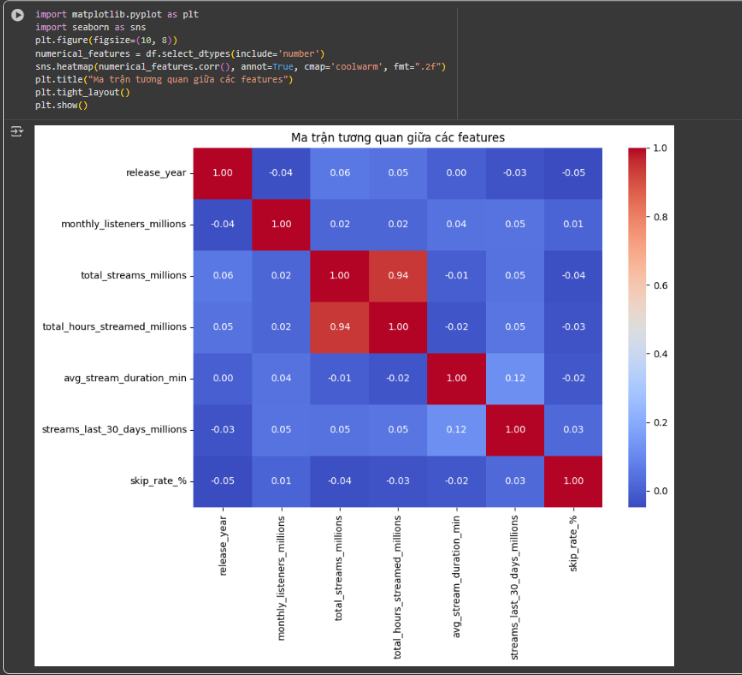
\includegraphics[width=1\linewidth]{../graphics/data2/3.png}
    \caption{Ma trận tương quan giữa các features}
    \label{fig:placeholder}
\end{figure}
Nhận xét:
\begin{itemize}
    \item Giữa total\_streams\_millions và total\_hours\_streamed\_millions có mối tương quan mạnh, hợp lý về mặt ý nghĩa vì khi số lượng stream tăng thì tổng giờ nghe cũng tăng tương ứng.
 \item Các hệ số của monthly\_listeners\_millions khá thấp so với các chỉ số khác, một nghệ sĩ có nhiều người nghe hàng tháng chưa chắc có tổng giờ stream cao( vì có thể mỗi người chỉ nghe 1-2 lần)
\item Tỉ lệ skip rate mặc dù có nhiều giá trị âm trong bảng tương quan không ảnh hưởng quá nhiều bởi các features khác, nó có thể liên quan nhiều hơn đến chất lượng nội dung hoặc sở thích cá nhân chứ không vì release\_year, nhiều nhạc cũ vẫn có thể hot nếu trở nên viral và nhạc mới ra chưa chắc đã nhiều người nghe.
\end{itemize}
\begin{figure}[H]
    \centering
    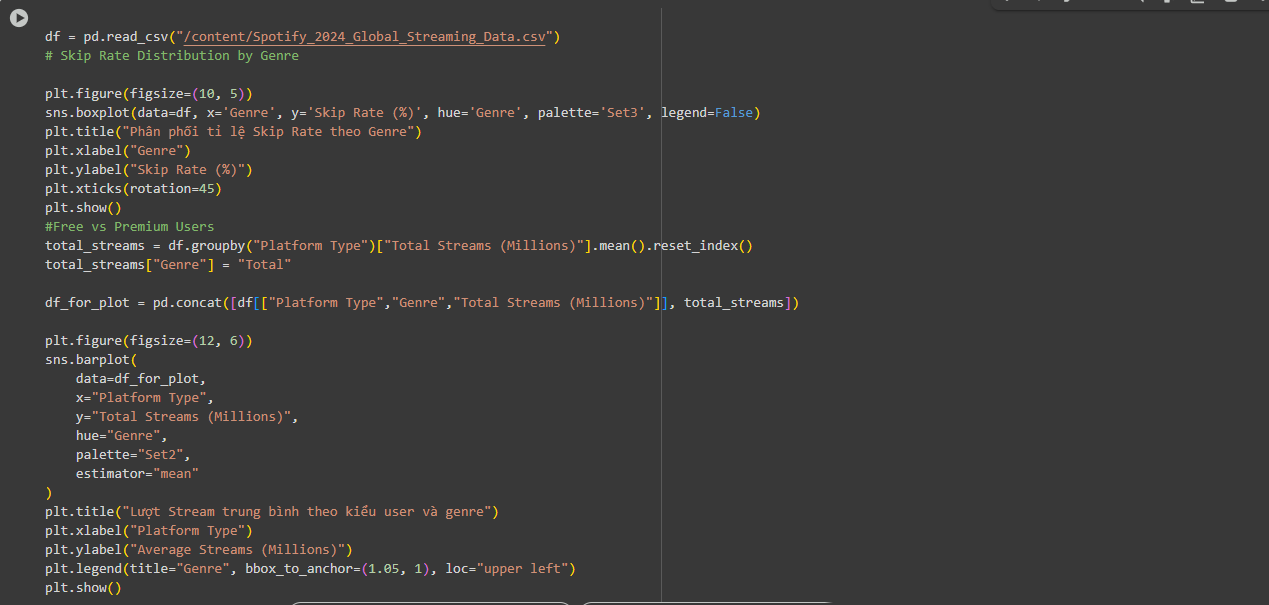
\includegraphics[width=1\linewidth]{../graphics/data2/11.png}
    \caption{Code thực thi}
    \label{fig:placeholder}
\end{figure}
\begin{figure}[H]
    \centering
    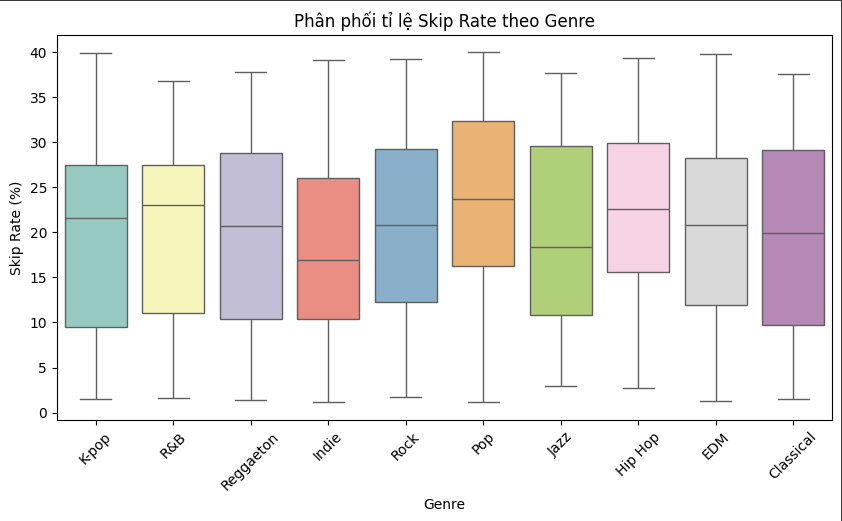
\includegraphics[width=1\linewidth]{../graphics/data2/12.png}
    \caption{Phân phối tỉ lệ Skip rate theo Genre}
    \label{fig:placeholder}
\end{figure}
\begin{figure}[H]
    \centering
    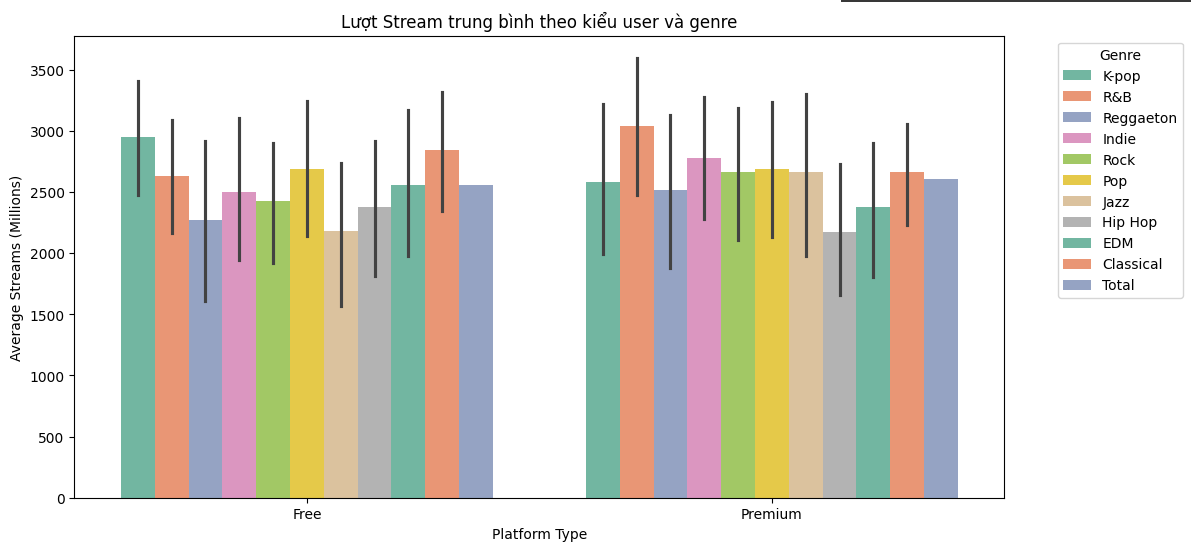
\includegraphics[width=1\linewidth]{../graphics/data2/13.png}
    \caption{Lượt Stream trung bình theo kiểu user và genre}
    \label{fig:placeholder}
\end{figure}

\textbf{Albums\_Info\_Clean.csv}
\\ Từ file csv thu được từ reccobeats, ta có được 1 số phân tích và cái nhìn tổng quan như sau:
\begin{figure}[H]
    \centering
    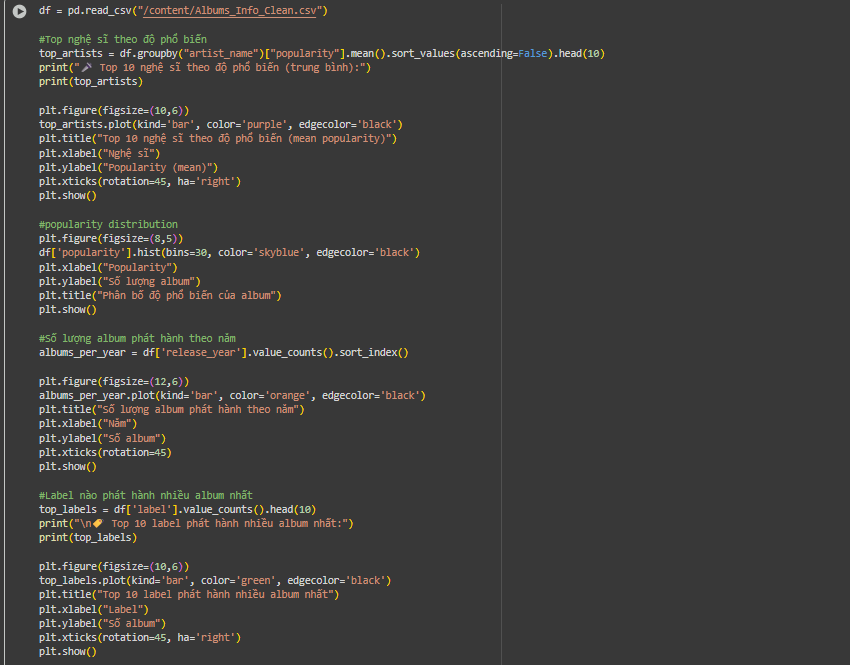
\includegraphics[width=0.8\linewidth]{../graphics/data2/6.png}
    \caption{Code thực thi}
    \label{fig:placeholder}
\end{figure}
\begin{figure}[H]
    \centering
    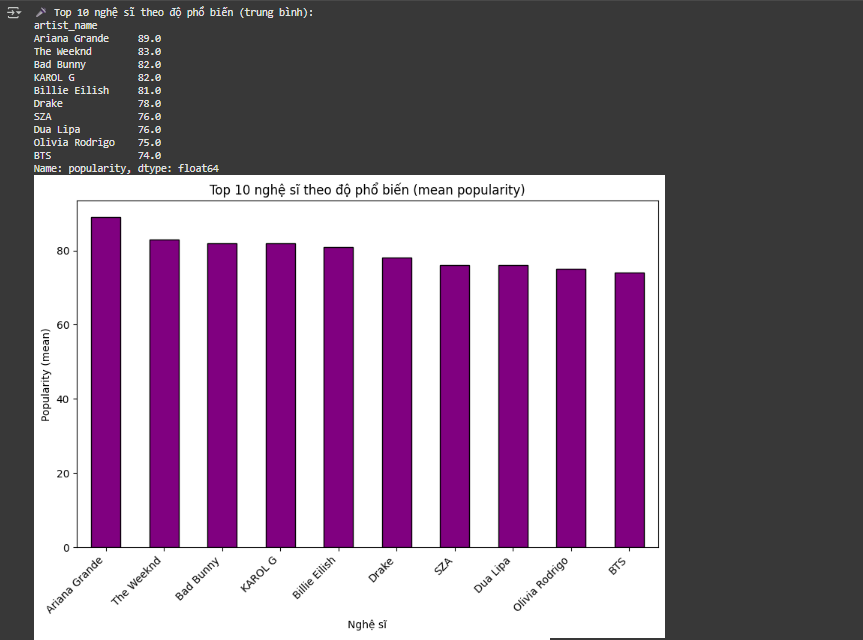
\includegraphics[width=0.7\linewidth]{../graphics/data2/7.png}
    \caption{Top 10 nghệ sĩ theo độ phổ biến}
    \label{fig:placeholder}
\end{figure}

\begin{figure}[H]
    \centering
    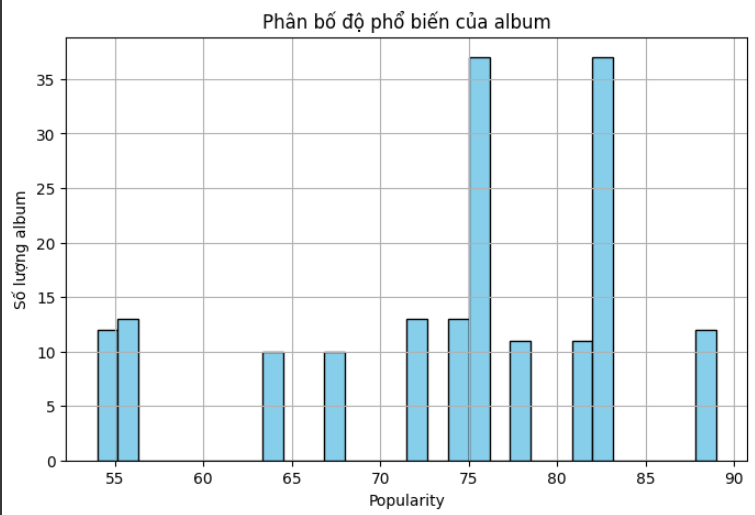
\includegraphics[width=0.7\linewidth]{../graphics/data2/8.png}
    \caption{Phân bố độ phổ biến của album}
    \label{fig:placeholder}
\end{figure}

\begin{figure}[H]
    \centering
    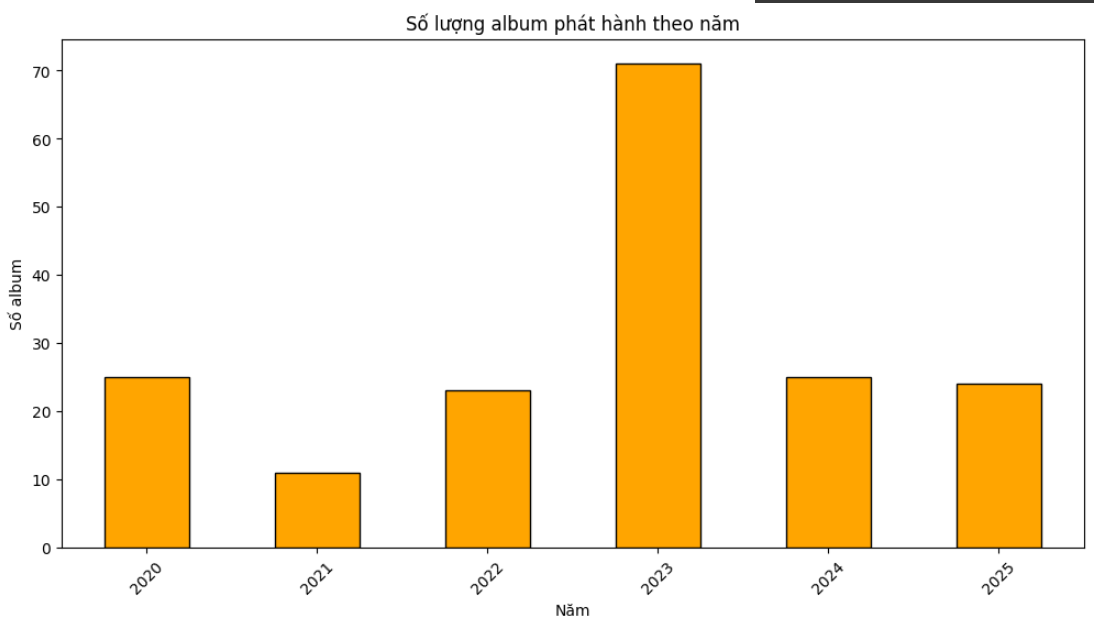
\includegraphics[width=0.7\linewidth]{../graphics/data2/9.png}
    \caption{Số lượng album phát hành theo năm}
    \label{fig:placeholder}
\end{figure}

\begin{figure}[H]
    \centering
    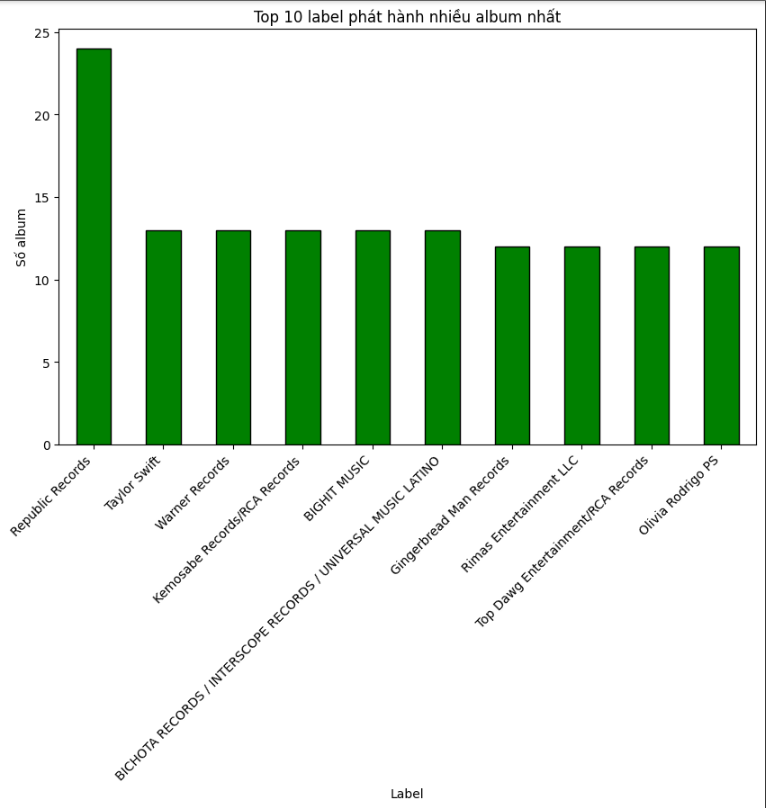
\includegraphics[width=0.7\linewidth]{../graphics/data2/10.png}
    \caption{Top 10 label phát hành nhiều album nhất}
    \label{fig:placeholder}
\end{figure}

\subsubsection{Mục tiêu:}
\begin{itemize}
    \item Với những gì dataset này cung cấp ta có thể thấy người dùng có tỷ lệ bỏ qua (skip rate) tăng và thời gian nghe giảm có thể được xem là rủi ro có thể rời bỏ nền tảng này hoặc không còm nhu cầu với premium. Kết hợp với lịch sử nghe nhạc, sở thích thể loại (genre preferences) và mức độ hoạt động trên ứng dụng, Spotify có thể dự đoán và ngăn chặn rủi ro rời bỏ bằng mô hình học máy.
    \item Dự đoán bài hát tiềm năng trở thành hit dựa trên skip rate,
thời gian nghe trung bình, số lượt stream ban đầu, mức độ lan truyền theo khu vực.
    \item Dự báo doanh thu dựa trên lượt stream trung bình và xu hướng theo thời gian, đề xuất nghệ sĩ hoặc thể loại nhạc phù hợp cho người dùng dựa trên hành vi nghe trước đó. 
    \item Xác định tần suất bỏ qua (skip rate) của từng thể loại → đo lường sự hấp dẫn của nhạc.

\end{itemize}
